\chapter{Results} 
\label{chap:results}
%\begin{enumerate}
%\item all data
%\item analysis done
%\item discussions
%\item comparisons
%\end{enumerate}
This section seeks to demonstrate the steps taken in the data gathering process, critical data analysis and validation of the effectiveness of models developed. We start by looking at fluid flows in the heart of the UWICSS and extracting parameters for models in Section~\ref{sec:windkessel_data}.  We can then demonstrate the effectiveness of the windkessel/lumped parameter model in predicting the behaviour of the aorta.  In validating the hydraulic system for the UWICSS, we also examine the effect of the mechanical delays for the valves and pumps.  These mechanical delays are a hindrance to the precise manipulation of fluid pressure and a direct limitation on the maximum frequency achievable by the controller.

This section also discusses the results drawn from the implementation of designs detailed in Chapter~\ref{chap:design}.  There are some important conclusions that can be made about the overall system and the numerical controller:
\begin{itemize}
\item The system based controller described in Chapter~\ref{chap:design}, is capable of achieving a maximum pulse frequency of 0.6 pulse per second.
\item The parameters of the two element windkessel model used in the system, can be successfully derived using known principles.
\item The current firmware architecture can be used to implement the numerical controller discussed in Section~\ref{sec:controller_design} of this thesis.
\item In order to achieve precise manipulation of fluid pressure between 0.4 pulse per second and a maximum of 6 pulses per second, faster actuations are required.
\item Comparison of the performance results between the system with mechanical delays and that of the system without these delays, shows the reduction in the performance of the controller.
\end{itemize}

\section{Results from Calibration of Sensors}

% chapter 3 the \texttt{x10abot_architecture_design_and_implementation (end)
%\chapter{Findings and Results} % (fold)
%\label{cha:findings_and_results}



\begin{figure}[H]
  \begin{center}
    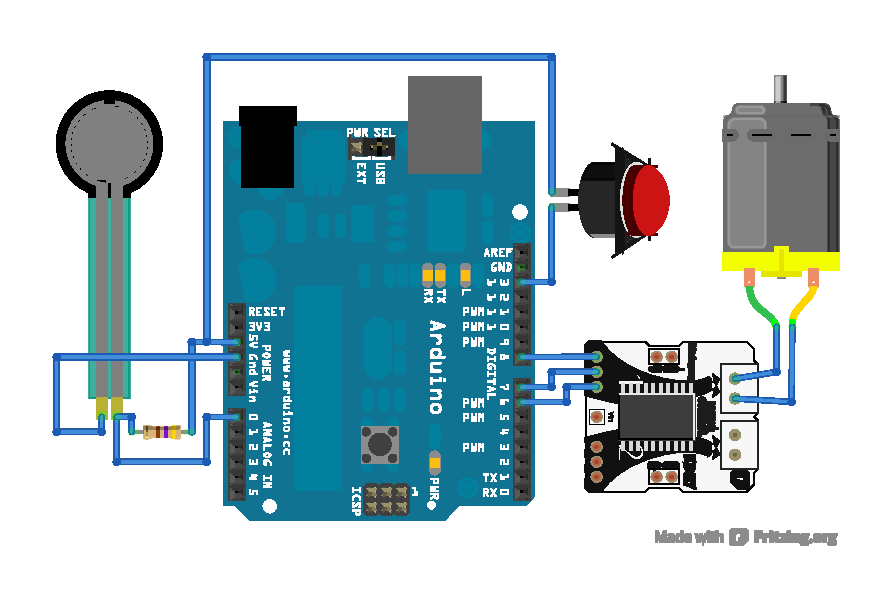
\includegraphics[width=1.0\columnwidth]{Figures/simple-example.pdf}
    \caption{The components of a simple singleboard \xten Example}
  \end{center}
\end{figure}

The following chapter demonstrates how the \xten architecture achieves its objectives through the hardware and software platform. We will demonstrate how the framework can be applied in a practical manner and we will explain the outcomes.

 We will demonstrate the framework in action by showing excerpts of sample programs for a simple mobile robot with a number of sensors and actuators distributed across one or more daughterboards.
%[mathescape,linenos, gobble=2,]


Code example~\ref{code:example} is a typical setup for a very simple mobile robot. All the sensors are on one daughterboard - in the case of our implementation, the ``internal'' daughterboard which is hosted on the same board as the motherboard. This robot has one actuator (a DC motor connected to an external H-bridge), a force sensor and a pushbutton sensor.


%\begin{multicols}{2}
	\begin{listing}[H]
		\footnotesize
		\begin{minted}[bgcolor=bg,frame=lines,framesep=2mm,label={\xten Sample code}]{c}

/**
* Import the necessary libraries for the motherboard, 
* daughterboard and the peripheral bus
**/
#include <Wire.h>  
#include <X10ABOT_MB.h>
#include <X10ABOT_DB.h> //Included to support the internal daughterboard #0

//Declare and initialize motor on daughterboard #0, actuator port #1
Actuator motor1(0,1);
//Declare  and initialize force sensor on daughterboard #0, sensor port #1
Sensor force1(0,1);
//Declare  and initialize force sensor on daughterboard #0, sensor port #2
Sensor pushbutton(0,1,B);

void setup(){}

void loop(){
//Continuously check the sensors for a reading
if(pushbutton.readDigital() || (force1.readAnalogue()>100)){
  motor1.on(100); //Turn motor1 on at full power (100%) 
  }else{
  motor1.off();  //Turn motor1 off
  }
}	 

		\end{minted}
		\caption{Example of the \xten architecture on a simple robot.} \label{code:example}
	\end{listing}
%	\vfill
%	\columnbreak



Code example~\ref{code:example} is a simple program that drives the motor in the forward(positive) direction at full speed if either the touch sensor records an input or if there is a force on the force sensor about a certain threshold, otherwise it will shut off the motors.

%\end{multicols}
In this instance, there are two types of devices that are declared, \textbf{Sensors} and \textbf{Actuators}. These represent the parent classes of all sensors and actuators respectively in the \xten architecture. All other sensor and actuator sub-types inherit from these two classes of devices, overriding where necessary.

It should be noted that it was necessary to include the library for both the motherboard and the daugterboard because the daughterboard and motherboard shares the same Arduino board. Daughterboard address \#0 is reserved for the internal or resident daugterboard on the same physical Arduino platform.

	\section{Modularity} % (fold)
	\label{sec:modularity}
% section modularity (end)
%Adding extra capability can be easily and seamlessly done using the \xten architecture. An extra daughterboard can represent a complete subsystem using sensors and actuators. A reasonable %example could be a simple robotic arm used to fetch items based on readings from one or more attached sensors. The \xten architecture allows for these new devices on separates %daughterboard to be attached via the perpheral bus. These modules can be just as easily added in software. Each daughterboard containing sensors and actuators can be declared with a unique %address similar to the existing modules. Instructions can then be added for its application.
 In the code example~\ref{code:modularity}, we see how an extra sensor and an actuator was added for an extra functionality. 

\begin{figure}[h!]
  \begin{center}
    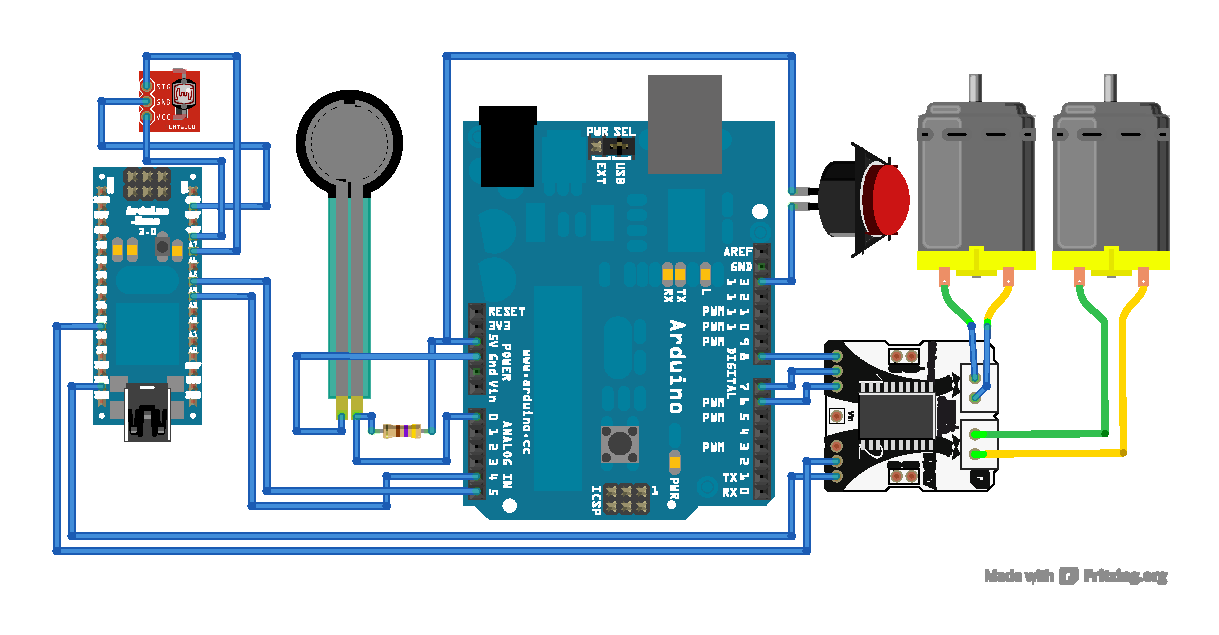
\includegraphics[width=1.0\columnwidth]{Figures/modular-example.pdf}
    \caption{The components of a Modular singleboard \xten Example}
  \end{center}
\end{figure}

\begin{listing}[H]
		\footnotesize
		\caption{Example of modularity in action.} \label{code:modularity}
		\begin{minted}[bgcolor=bg,frame=lines,framesep=2mm,label={Modularity in Code}]{c}
/**
* Import the necessary libraries for the motherboard, 
* daughterboard and the peripheral bus
**/
#include <Wire.h>  
#include <X10ABOT_MB.h>
#include <X10ABOT_DB.h> //Included to support the internal daughterboard #0

//Declare motor on daughterboard #0, actuator port #1
Actuator motor1(0,1);
//Declare force sensor on daughterboard #0, sensor port #1
Sensor force1(0,1);
//Declare force sensor on daughterboard #0, sensor port #2
Sensor pushbutton(0,1,B);
//Declare motor on daughterboard #9, actuator port #1
Actuator motor2(9,1);
//Declare force sensor on daughterboard #9, sensor port #1
Sensor lightSensor(9,5);

void setup(){}
void loop(){
//Continuously check the sensors for a reading
if(pushbutton.readDigital || force1.readAnalogue()){
  motor1.on(100); //Turn motor1 on at full power (100%) 
}else{
  motor1.off();  //Turn motor1 off
  }
//Added extra functionality with a new sensor and a new actuator on daughterboard #9
//while motor1 is running and light is on the sensor, activate motor2
if (motor1.isOn() && lightSensor.readAnalogue())
  {motor2.on(-50); //Turn motor2 on at 50% in the reverse direction
  }else{
  motor2.off();  //Turn motor2 off
  }
}	 
	\end{minted}
		
\end{listing}
In this particular example (code~\ref{code:modularity}), even though \emph{motor1} and \emph{lightSensor}, two additional, independent devices were added to the system, it did not affect the existing code but fit seamlessly in the development process. Separate code was added to carry out its operation which never needed to interact with the exisiting system. There needed to be no special acccomodation for the new module in the existing system. There also was no hardware modification made to the existing setup even with the fact that an extra physical component, another daughterboard, was added to the system.
All these features are an indication of a truly modular architecture. As previously defined, we included an entire subsystem without modifying the existing components. The modules can be removed just as easy as they were installed. The level of expertise required to modify this system is also relatively minimal due to its design.


% chapter findings_and_results (end)
\section{Extensibility and Abstraction} % (fold)
\label{sec:extensibility_abstraction}
We demonstrate the \xten architecture's ability to support new and varied types of sensors and actuators. This is accomplished with no knowledge of the low-level details of the hardware.
In the following example, we will define a simple, yet complete library that reads and interprets the data from a thermistor temperature sensor. The temperature value will be returned in fahrenheit units. This code was sourced from the Arduino Playground \cite{therm} as a simple example to acquire thermistor temperature readings. We made a simple modification that allowed the same code to be applicable to the \xten architecture.
\begin{listing}[H]
		\footnotesize
		\caption{Example: A complete library for a thermistor temperature sensor.} \label{code:therm}
		\begin{minted}[bgcolor=bg,frame=lines,framesep=2mm,label={Thermistor Library}]{c}
#include <Sensor.h>
#include <math.h>

double readThermister() {
 int RawADC = analog(_db,_port);
 double Temp;
 Temp = log(((10240000/RawADC) - 10000));
 Temp = 1 / (0.001129148 + (0.000234125 + (0.0000000876741 * Temp * Temp ))* Temp );
 Temp = Temp - 273.15;            // Convert Kelvin to Celcius
 Temp = (Temp * 9.0)/ 5.0 + 32.0; // Convert Celcius to Fahrenheit
 return Temp;
}
	\end{minted}
		
\end{listing}

The library in code example \ref{code:therm} above is an almost exact replica of the fragment of code extracted from the Arduino library. The code accesses the analogue pin to read the sensor. The \xten framework possesses special functions that access hardware components. For this particular case, the \textbf{analog(\_db,\_port)} function was invoked. This is a method used to abstract the analog pin so it becomes hardware independent. The analogue pin here is perceived as a virtual entity that belongs on a daughterboard \textbf{\_db} on a particular port \textbf{\_port}. The result is then returned to the calling function, presenting the temperature value to the user in Fahrenheit.

This thermistor library can then be easily utilized by the user as follows:

The code in code example~\ref{code:thermcode} presents a temperature monitoring system that watches the temperature that it receives from two thermistors. If the value read from the thermistors goes beyond particular thresholds for either of them, an alarm is triggered.
\begin{listing}[H]
		\footnotesize
		\caption{Example application of the thermistor temperature sensor library.} \label{code:thermcode}
		\begin{minted}[bgcolor=bg,frame=lines,framesep=2mm,label={Thermistor Example Application}]{c}
#include <Wire.h>  
#include <Thermistor.h>  
#include <X10ABOT_MB.h>

//Declare motor on daughterboard #17, actuator port #1
Thermistor temp1(17,1);
//Declare force sensor on daughterboard #108, sensor port #6
Thermistor temp2(108,6);
//Declare digital alarm on daughterboard #10, sensor port #3
Buzzer alarm(10,3,A);

void setup(){}
void loop(){
//Continuously check the sensors to see if temperature within threshold
  if((temp1.readThermister() > 70 )|| temp1.readThermister()<30){
  alarm.on(); //Turn on alarm 
}
	\end{minted}
		
\end{listing}

The library for was included and it became pretty straightforward to manipulate the sensor afterwards.
% section extensibility and abstraction (end)

\section{Scalability} % (fold)
\label{sec:scalability}

% section scalability (end)
The results for the application on modularity are two fold and can be seen clearly to imply scalability. The method of modular additions is scalable to tens of modules as defined by the peripheral bus protocol. We therefore need to benchmark the performance of the architecture implemented on the Arduino platform. This is necessary to evaluate the speed at which instructions are excuted. This can determine how the system will perform when under duress from multiple hardware devices simultaneously. These statistics can then be evaluated to deduce the architecture's suitability for a particular project. The \xten architecture's major limiting factor is the speed of the peripheral bus, however, other hardware specific limitations may come into play. These may include, clock speed and available RAM, all of which may differ, even across Arduino hardware platforms. All tests below were carried out on the Arduino Mega, using the Atmel \texttrademark ATMega1280 microcontroller.

We carried out a few timing tests to evaluate the performance of the \xten framework on the Arduino platform. The test were done using one motherboard and three daughterboards. The typical robotics project may never require as many daughter boards since one Arduino Mega may support up to eight sensor ports and six actuator ports. The smaller Arduino Uno can support up to three sensor ports and two actuator ports. Any combination of one or more of these Arduino boards can be used to implement the \xten architecture.
We did timing tests to measure the latency between the command request and the response. We also recorded the measurable difference when the peripheral bus is congested with a rapid succession of events for all the six daughterboards.

The tables below display the results of our timing experiments, the timing utility on the Arduino has a maximum resolution of 4 micro second intervals.

\begin{table}[h!]
    %\scriptsize {
	%\centering
	\caption{Table showing microcode latency in microseconds($\mu$s) on the on-board daughteroard over 20 consecutive executions.}
	\begin{tabular}{|l|l|l|l|}
	\toprule
 \multicolumn{4}{c}{\textbf{ONBOARD daughterboard}} \\\hline

digitalOut & digitalIn & pwm & analogue \\\hline
40 & 50084 & 60 & 50212\\\hline
40 & 50088 & 60 & 50216 \\\hline
40 & 50084 & 60 & 50212 \\\hline
36 & 50084 & 60 & 50216 \\\hline
40 & 50084 & 56 & 50212 \\\hline
40 & 50084 & 60 & 50212 \\\hline
40 & 50084 & 60 & 50212 \\\hline
40 & 50080 & 60 & 50216 \\\hline
40 & 50084 & 60 & 50216 \\\hline
48 & 50080 & 56 & 50216 \\\hline
40 & 50088 & 56 & 50216 \\\hline
40 & 50084 & 56 & 50216 \\\hline
40 & 50084 & 60 & 50216 \\\hline
36 & 50084 & 60 & 50216 \\\hline
40 & 50080 & 60 & 50220 \\\hline
40 & 50084 & 64 & 50216 \\\hline
40 & 50084 & 56 & 50216 \\\hline
40 & 50080 & 60 & 50224 \\\hline
40 & 50084 & 56 & 50216 \\\hline
\multicolumn{4}{c}{Average Times} \\\hline
40.00 & 50083.58 & 58.95 & 50215.58

%}
\end{tabular}
\end{table}

The latency for output operations was significantly less time than that of input operations. This was expected since there is no waiting period to request the value of the data from the port on the daughterboard for output operations.  

\begin{table}[H]
    %\scriptsize {%
	\centering
	\caption{Table showing microcode latency in microseconds($\mu$s) on the off-board daughteroard over 20 consecutive executions.}
	
	\begin{tabular}{|l|l|l|l|}
	\toprule
 \multicolumn{4}{c}{\textbf{OFFBOARD daughterboard}} \\\hline
digitalOut & digitalIn & pwm & analogue\\\hline
568 & 51320 & 688 & 51328\\\hline
560 & 51320 & 684 & 51320\\\hline
568 & 51324 & 684 & 51324\\\hline
568 & 51324 & 684 & 51328\\\hline
568 & 51332 & 684 & 51324\\\hline
564 & 51324 & 684 & 51332\\\hline
564 & 51324 & 684 & 51328\\\hline
564 & 51320 & 688 & 51324\\\hline
564 & 51320 & 680 & 51332\\\hline
568 & 51324 & 688 & 51324\\\hline
564 & 51324 & 680 & 51324\\\hline
568 & 51324 & 684 & 51324\\\hline
564 & 51320 & 684 & 51328\\\hline
568 & 51328 & 684 & 51324\\\hline
560 & 51320 & 688 & 51328\\\hline
564 & 51320 & 688 & 51328\\\hline
568 & 51324 & 684 & 51332\\\hline
564 & 51320 & 684 & 51324\\\hline
564 & 51320 & 684 & 51324\\\hline
\multicolumn{4}{c}{Average Times} \\\hline
565.26 & 51322.74 & 684.63 & 51326.32

%}
\end{tabular}
\end{table}

We carried out an experiment to determine how the system performed when executing a barrage of instruction and obtained the results lsted in table X below. 
\begin{table}[H]
    %\scriptsize {%
	\centering
	\caption{Table showing microcode latency in microseconds($\mu$s) on the off-board daughteroard for number of instructions executed(no.) and associated time it took to complete over 5050 consecutive executions of digitalOut.}
	
	\begin{tabular}{|l|l||l|l||l|l||l|l||l|l||}
	\toprule
 \multicolumn{10}{c}{\textbf{OFFBOARD daughterboard barrage}} \\\hline


no. & time ($\mu$s)& no. & time ($\mu$s)& no. & time ($\mu$s)& no. & time ($\mu$s)& no. & time ($\mu$s) \\\hline
1 & 568 & 21 & 11840 & 41 & 23120 & 61 & 34380 & 81 & 45648 \\\hline
2 & 1132 & 22 & 12412 & 42 & 23676 & 62 & 34936 & 82 & 46216 \\\hline
3 & 1696 & 23 & 12972 & 43 & 24244 & 63 & 35516 & 83 & 46780 \\\hline
4 & 2268 & 24 & 13524 & 44 & 24796 & 64 & 36080 & 84 & 47352 \\\hline
5 & 2820 & 25 & 14108 & 45 & 25364 & 65 & 36620 & 85 & 47916 \\\hline
6 & 3384 & 26 & 14656 & 46 & 25932 & 66 & 37208 & 86 & 48480 \\\hline
7 & 3948 & 27 & 15228 & 47 & 26484 & 67 & 37772 & 87 & 49044 \\\hline
8 & 4520 & 28 & 15788 & 48 & 27068 & 68 & 38332 & 88 & 49600 \\\hline
9 & 5072 & 29 & 16352 & 49 & 27620 & 69 & 38880 & 89 & 50172 \\\hline
10 & 5636 & 30 & 16908 & 50 & 28188 & 70 & 39456 & 90 & 50736 \\\hline
11 & 6212 & 31 & 17472 & 51 & 28760 & 71 & 40028 & 91 & 51296 \\\hline
12 & 6768 & 32 & 18044 & 52 & 29316 & 72 & 40588 & 92 & 51860 \\\hline
13 & 7332 & 33 & 18600 & 53 & 29872 & 73 & 41156 & 93 & 52420 \\\hline
14 & 7896 & 34 & 19172 & 54 & 30452 & 74 & 41696 & 94 & 52980 \\\hline
15 & 8460 & 35 & 19732 & 55 & 31008 & 75 & 42276 & 95 & 53552 \\\hline
16 & 9020 & 36 & 20300 & 56 & 31552 & 76 & 42844 & 96 & 54112 \\\hline
17 & 9584 & 37 & 20856 & 57 & 32140 & 77 & 43408 & 97 & 54672 \\\hline
18 & 10148 & 38 & 21424 & 58 & 32696 & 78 & 43976 & 98 & 55244 \\\hline
19 & 10708 & 39 & 21988 & 59 & 33248 & 79 & 44536 & 99 & 55804 \\\hline
20 & 11280 & 40 & 22548 & 60 & 33828 & 80 & 45096 & 100 & 56364 \\\hline
\multicolumn{10}{c}{Total time taken: 2847984} \\\hline
\end{tabular}
\end{table}
 The results showed that even at high instruction thoroughput, the time to execute a particular instruction does not vary significantly from its latency as a single instruction.


\section{Economy} % (fold)
\label{sec:economy}

% section economy (end)
